%%=========================================
\chapter{Results and Discussion}\label{ch:results-and-discussion}
In this chapter, experimental results are presented, analysed, and discussed. In total, one (111)B substrate from vendor A (substrate A), two (111)B substrates from vendor B (substrate B and substrate B2), and one (211)B substrate from vendor A (substrate C) were investigated using bright and dark field microscopy, \ac{sem}, \ac{eds}, \ac{afm}, near-\ac{ir} transmission microscopy, and \ac{ftir}. The substrates were investigated both as-received and after surface pre-growth preparation, except substrate B2, which was was not investigated as-received. As the final step, \iac{mct} film was grown on each substrate, except the shattered substrate B, and the same characterisation as for the substrates was conducted to correlate the number of defects and the type of defects in the grown \ac{mct} layer with the preparation of the substrate.
%%=========================================
\section{Surface Analysis of As-Received Substrate A}\label{sec:subAa}
% Substrate A
In previous work \citep{lauten2017characterisation}, the state-of-the-art as-received (111)B-oriented substrate A was characterised for polishing damage, defects, and residual particles using optical microscopy, \ac{sem} with \ac{eds}, and \ac{xps}. The results are\andreas{/were} reiterated in this section to better present the full scope of the study. In addition to the previously used methods, \ac{afm}, near-\ac{ir} transmission microscopy, and \ac{ftir} were used to study the as-received substrate.

\begin{figure}[htbp]
    \centering
    \mySubfigure{\linewidth}{LM_DF_BZ1503ID71A_M005_centre.jpg}[fig:subAa_om_df_centre]
    \par\bigskip
    \mySubfigure{0.4525\textwidth}{LM_DF_BZ1503ID71A_M005_edge.jpg}[fig:subAa_om_df_edge]
    \hfill
    \mySubfigure{0.5225\textwidth}{LM_DF_BZ1503ID71A_M005_corner_with_skraa.jpg}[fig:subAa_om_df_corner]
    \caption[Dark field images of substrate A.]{Dark field images of substrate A captured through the optical microscope Leica DM RXA2 at three different locations on the substrate surface: \subref{fig:subAa_om_df_centre} Centre; \subref{fig:subAa_om_df_edge} edge; and \subref{fig:subAa_om_df_corner} corner.}
    \label{fig:subAa_om_df}
\end{figure}

Dark field images from the surface of substrate A at the corner, edge, and centre of the substrate, see Fig.~\ref{fig:subAa_om_df}, show that the highly polished (111)B surface was smooth and with only a few particles or morphological defects. The particle and morphological defect density was estimated to be \SI{4e2}{\centi\metre^{-2}} at the centre and \SI{1e3}{\centi\metre^{-2}} at the edges and corners of the surface of substrate A. Here the particle and morphological defect density refers to the sum of all light scattering objects with sizes \SI{>0.5}{\micro\metre} since any particles or morphological defects that have sizes \SI{<0.5}{\micro\metre} were not seen in the dark field images. Therefore, the true morphological defect density was higher than the one estimated from the dark field images.
% --- Measured with tolerance of 7 using ImageJ.
%       Centre: 17 partikler på 2048x1536
%       Corner: 30 partikler på 1732x1327

The substrates from vendor A were considered to be state-of-the-art \ac{czt} substrates. They were fine-polished by the vendor, and consequently, they had few surface features. This made it challenging to focus the \ac{sem} and find particles on the surface. At a magnification of $100\times$, no particles or defects could be seen, see Fig.~\ref{fig:EDX_BZ1503A_a_m001}. As a result of a higher occurrence of particles towards the edges of the substrate, it was easier to find focus near the edges. An area from the left edge of the substrate with 12 bright spots and three dark vertical lines were observed in Fig.~\ref{fig:substrateA_a2_m005}. The dark, vertical lines were carbon contamination from the \ac{sem} and was not studied further. The bright spots corresponded to an irregularity or particle on the surface. These features will be described in the following by, among other methods, high-resolution \ac{sem} images and \ac{eds} spectra.

\begin{figure}[htbp]
    \centering
    \mySubfigure{0.49\linewidth}{EDX_BZ1503A_a_m001.jpg}[fig:EDX_BZ1503A_a_m001]
    \hfill
    \mySubfigure{0.49\linewidth}{substrateA_a2_m005.jpg}[fig:substrateA_a2_m005]
    \caption[\Ac{sem} images of substrate A.]{\Ac{sem} images of the surface of substrate A taken near the left edge at \subref{fig:EDX_BZ1503A_a_m001} low ($100\times$) and \subref{fig:substrateA_a2_m005} high magnification ($3500\times$).}
    \label{fig:subA_overview}
\end{figure}
% A particle and morphological defect density of features \SI{>0.5}{\micro\metre} of \SI{4e2}{\centi\metre^{-2}} at the centre and \SI{1e3}{\centi\metre^{-2}} at the edges of the substrate was observed. Substrate A had polishing scratches that were between 10 and \SI{20}{\nano\metre} wide. In addition, pieces of residual polishing grit was found on the surface. An \ac{eds} spectrum of an agglomeration of multiple particles revealed that they were composed of alumina (\ce{Al2O3}) and silica (\ce{SiO2}) polishing grit. In addition, larger particles with size of \SI{\sim 10}{\micro\metre} on the substrate surface were observed. \Ac{eds} revealed that these particles mainly consisted of titanium.

%%=========================================
\subsection{Particles}
There were so few particles on substrate A that it was difficult to determine a density of particles on this substrate. The surface was so uniform that it was difficult to keep in focus even at high magnification. However, four different types of particles were found and identified on the surface of substrate A, as seen in Fig.~\ref{fig:subAa_sem_w_eds}.

\begin{figure}
    \centering
    \begin{subfigure}[t]{\textwidth}
        \caption{}\label{fig:subAa_polishing-grit}
          \begin{minipage}[t]{0.43\linewidth}
            \centering
            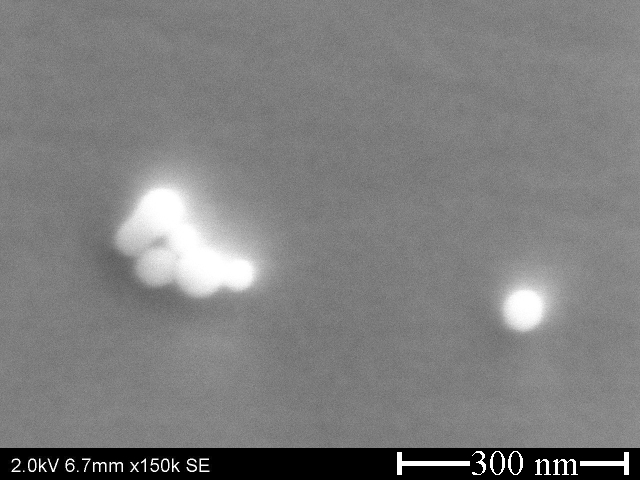
\includegraphics[width=\linewidth]{substrateA_a2_m006.jpg}
          \end{minipage}
          \hfill
          \begin{minipage}[t]{0.43\linewidth}
            \centering
            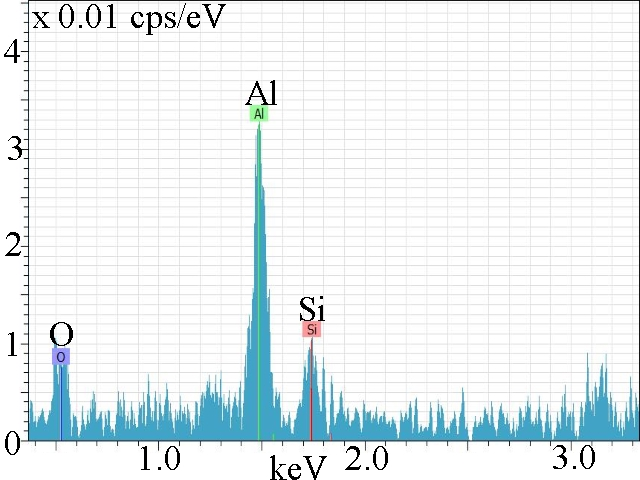
\includegraphics[width=\linewidth]{subA_eds_alumina02.jpg}
          \end{minipage}
          \begin{minipage}[t]{0.11\linewidth}
            \centering
            \atomicTable[&][&][&]
          \end{minipage}
    \end{subfigure}
    \par\bigskip
    \begin{subfigure}[t]{\textwidth}
        \caption{}\label{fig:subAa_large-grit}
          \begin{minipage}[t]{0.43\linewidth}
            \centering
            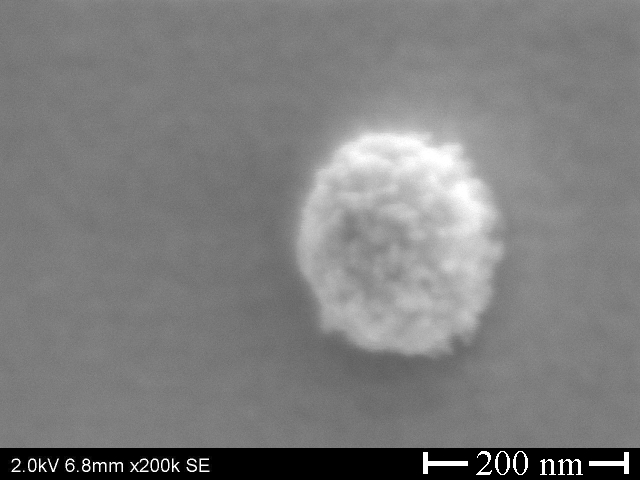
\includegraphics[width=\linewidth]{substrateA_a1_m016.jpg}
          \end{minipage}
          \hfill
          \begin{minipage}[t]{0.43\linewidth}
            \centering
            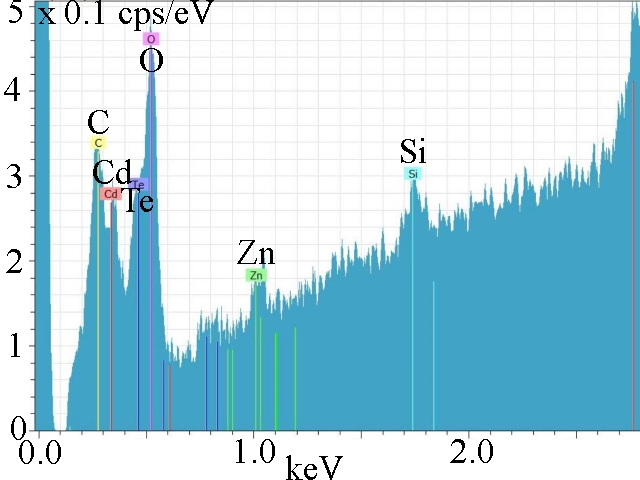
\includegraphics[width=\linewidth]{eds_subA_SiO2.jpg}
          \end{minipage}
          \begin{minipage}[t]{0.11\linewidth}
            \centering
            \atomicTable[&][&][&]
          \end{minipage}
    \end{subfigure}
    \par\bigskip
    \begin{subfigure}[t]{\textwidth}
        \caption{}\label{fig:subAa_czt-particle}
          \begin{minipage}[t]{0.43\linewidth}
            \centering
            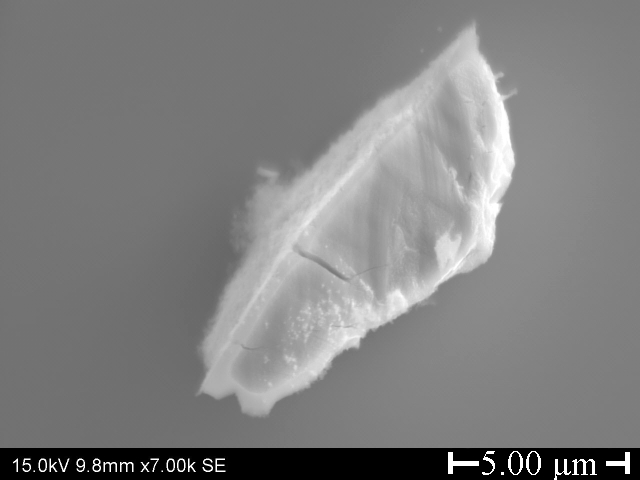
\includegraphics[width=\linewidth]{substrateA_a2_m011.jpg}
          \end{minipage}
          \hfill
          \begin{minipage}[t]{0.43\linewidth}
            \centering
            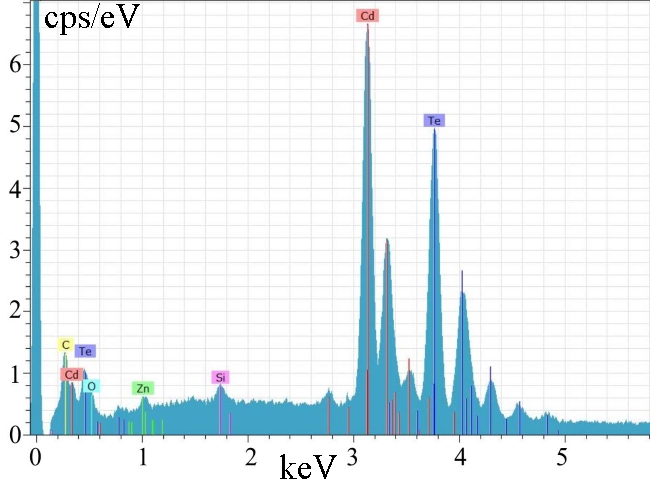
\includegraphics[width=\linewidth]{eds_subA_CZT.jpg}
          \end{minipage}
          \begin{minipage}[t]{0.11\linewidth}
            \centering
            \atomicTable[&][&][&]
          \end{minipage}
    \end{subfigure}
    \caption[\Ac{sem} images, \ac{eds} spectra, and \ac{eds} atomic compositions of four different types of particles found on as-received substrate A.]{High resolution \ac{sem} images of four different types of particles found on the as-received substrate A and the corresponding \ac{eds} spectra and atomic compositions: \subref{fig:subAa_polishing-grit} Alumina (\ce{Al2O3}) and silica (\ce{SiO2}) polishing grit; \subref{fig:subAa_large-grit} silicon carbide (\ce{SiC}) and silica (\ce{SiO2}); \subref{fig:subAa_czt-particle} \aca{czt} (\ce{Cd_{0.96}Zn_{0.04}Te}) particle; and \subref{fig:subAa_titanium-particle} titanium (\ce{T}) particle.}\label{fig:subAa_sem_w_eds}
\end{figure}

\begin{figure}[htbp]
\ContinuedFloat
    \centering
    \begin{subfigure}[t]{\textwidth}
        \caption{}\label{fig:subAa_titanium-particle}
          \begin{minipage}[t]{0.43\linewidth}
            \centering
            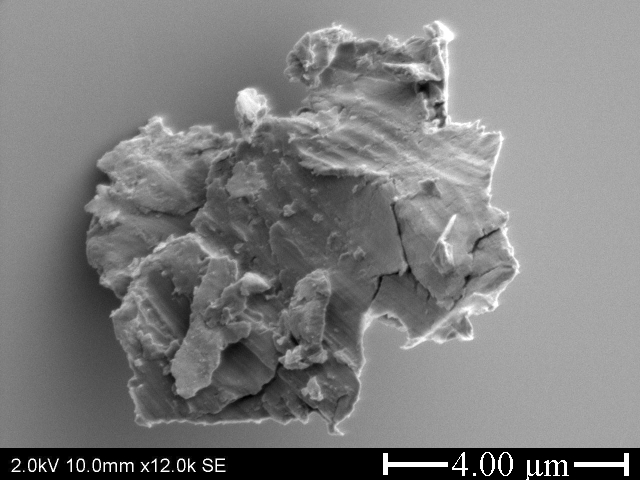
\includegraphics[width=\linewidth]{titan_sem.jpg}
          \end{minipage}
          \hfill
          \begin{minipage}[t]{0.43\linewidth}
            \centering
            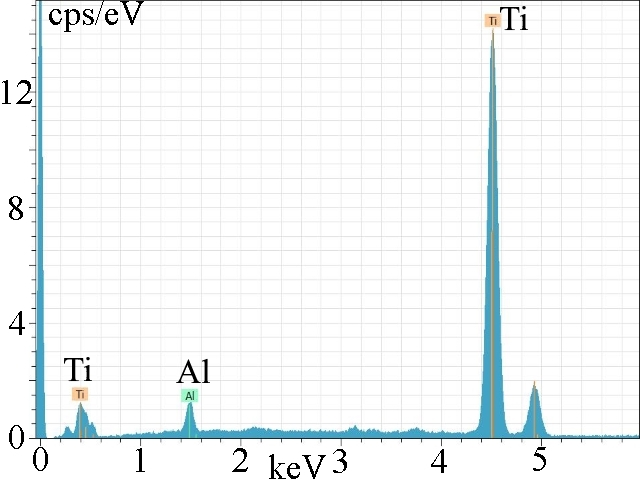
\includegraphics[width=\linewidth]{titan_eds.jpg}
          \end{minipage}
          \begin{minipage}[t]{0.11\linewidth}
            \centering
            \atomicTable[&][&][&]
          \end{minipage}
    \end{subfigure}
    \captionsetup{list=no}
    \caption{\emph{(continued)}}
\end{figure}

%%=====
\subsubsection{Alumina (\ce{Al2O3}) and Silica (\ce{SiO2}) Polishing Grit}
Small particles of size \SI{50}{\nano\metre} were observed near the edges of substrate A, see Fig.~\ref{fig:subAa_polishing-grit}. The \ac{sem} image shows an agglomeration of particles and one single particle with a diameter of \SI{50}{\nano\metre}. The large piece was an agglomeration of the smaller ones. The corresponding \ac{eds} spectrum of the large piece revealed that the particles consisted of \ce{Al}, \ce{Si} and \ce{O}. The particles were most likely residual \ce{Al2O3} and \ce{SiO2} polishing grit which are commonly used in polishing slurries \citep{benson2015as-received}. 

It seemed like the polishing grits were easier to observe in close proximity to the edges of the substrate and consequently had a higher density towards the edges than further in towards the centre, but this could also be due to the difficulties of focusing the \ac{sem} beam on the flat surface. 

The upper limit on the polishing grit density close to the edges of the substrate was estimated from Fig.~\ref{fig:substrateA_a2_m005} to be \SI{3e6}{\particle\centi\metre^{-1}}. It was not possible to get any sharp \ac{sem} images to count the density of polishing grit further in on the substrate, but it could be assumed that the density further in was smaller than \SI{3e6}{\particle\centi\metre^{-1}}.

%%=====
\subsubsection{Silicon Carbide (\ce{SiC}) and Silica (SiO2)}
A particle with a diameter of \SI{200}{\nano\metre} is shown in Fig.~\ref{fig:subAa_large-grit} with the corresponding \ac{eds} spectrum. This particle was considerably larger and had a rougher surface than the more frequently observed \SI{50}{\nano\metre} particles that were found to be residual polishing grit. The \ac{eds} spectrum of the particle revealed that the particle consisted of \ce{Si}, \ce{C}, and \ce{O}, which indicated that this particle could be residual \ce{SIO2} polishing grit, \ce{SiC} polishing grit, or an agglomeration of both. \todo{Finn atomprosent for å avgjøre. SiC eller SiO2? Hvor kommer C fra hvis bare SiO2?}


%%=====
\subsubsection{CZT}
Particles with size \SI{>5}{\micro\metre} were observed primarily near the edges of substrate A. Fig.~\ref{fig:subAa_czt-particle} shows a particle that was \SI{13}{\micro\metre} long and \SI{5}{\micro\metre} wide. A comparison between the corresponding \ac{eds} spectrum of the particle and the substrate surface spectrum revealed that the particle consisted of the same material as the underlying substrate. It could be debris from the cutting and polishing of the substrate by the vendor.


%%=====
\subsubsection{Titanium}
Particles with sharp edges and sizes of \SI{>5}{\micro\metre} were observed in the upper left corner of the substrate. The particles appeared darker than the \ac{czt} particles in \ac{sem} and with more edges. Fig.~\ref{fig:subAa_titanium-particle} shows a particle that was \SI{8}{\micro\metre} long and \SI{4}{\micro\metre} wide. The corresponding \ac{eds} spectrum of the particle revealed that the particle mainly consisted of titanium. The sharp edges indicate that the particle had not not been used as polishing grit because the edges had been rounded in that case. Unfortunately, these particles probably had settled on the substrate during the study. A new substrate holder was made for \ac{xps} measurements out of titanium in the machine shop. When mounting the substrate in the holder with a screw, some titanium particles were made. However, they were confined to a small area in the upper left corner of the substrate. \Ac{sem} and \ac{eds} measurements of particles from the \ac{xps} holder, collected with an adhesive carbon tab, confirms that the same type of titanium particles were found on the \ac{xps} holder. %This fact, shows how important it is to clean the equipment carefully before use. %see Fig.~\ref{fig:subAa_titanium}


%%=========================================

\subsection{Surface Scratches and Roughness}
The as-received surface of substrate A was carefully polished by the vendor, as seen in Fig.~\ref{fig:subAa_scratches}. The surface scratches most likely have shallow depth since they could not be seen in the dark field images of substrate A, see Fig.~\ref{fig:subAa_om_df}.

\begin{figure}[htbp]
    \centering
    %\subfigure[High resolution SEM at SEM image at a magnification of 80000$\times$.]{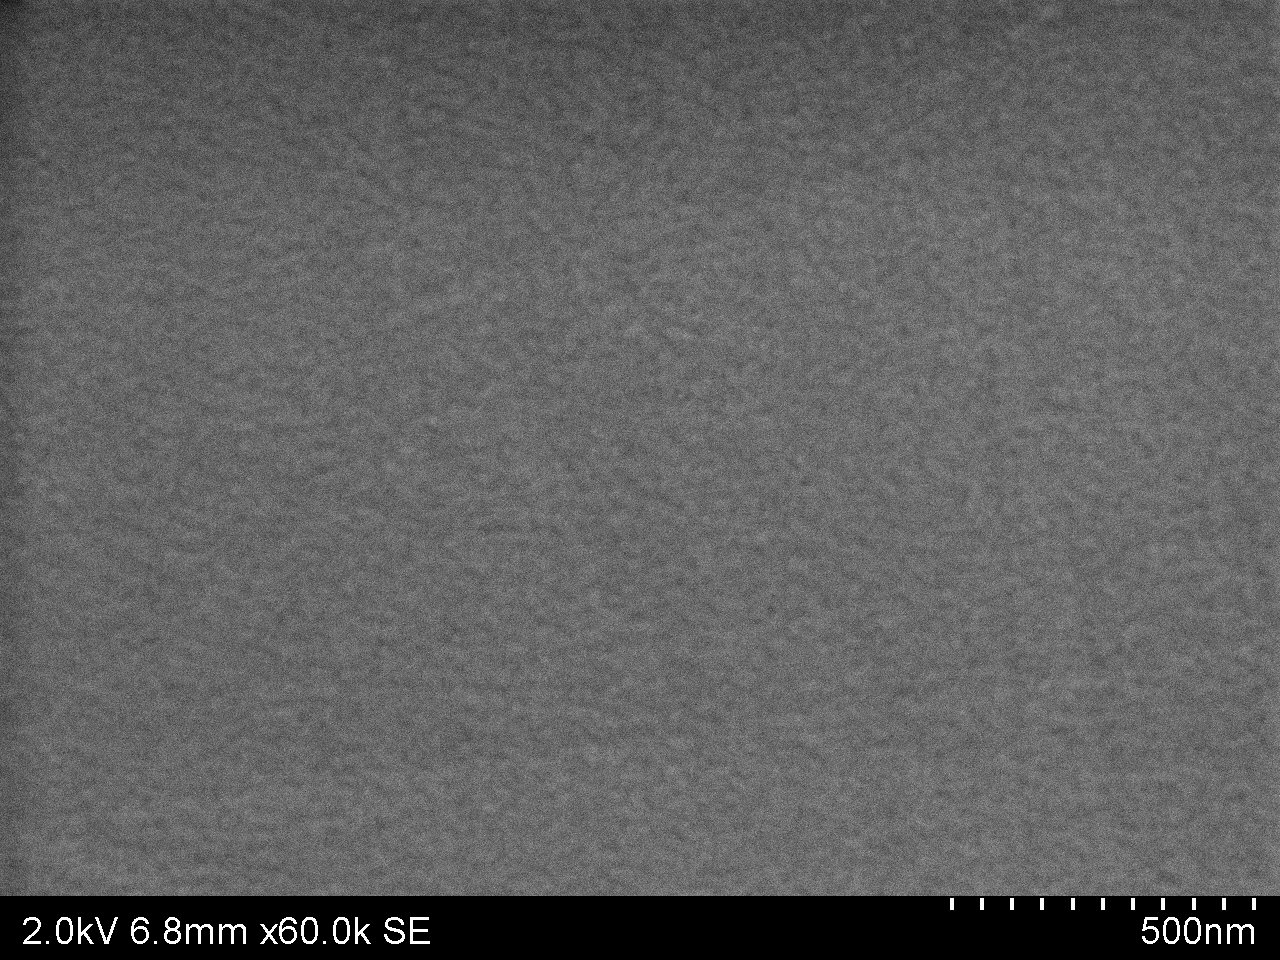
\includegraphics[width=0.48\linewidth]{substrateA_a2_m003.jpg}\label{fig:substrateA_a2_m003}}
    %\quad
    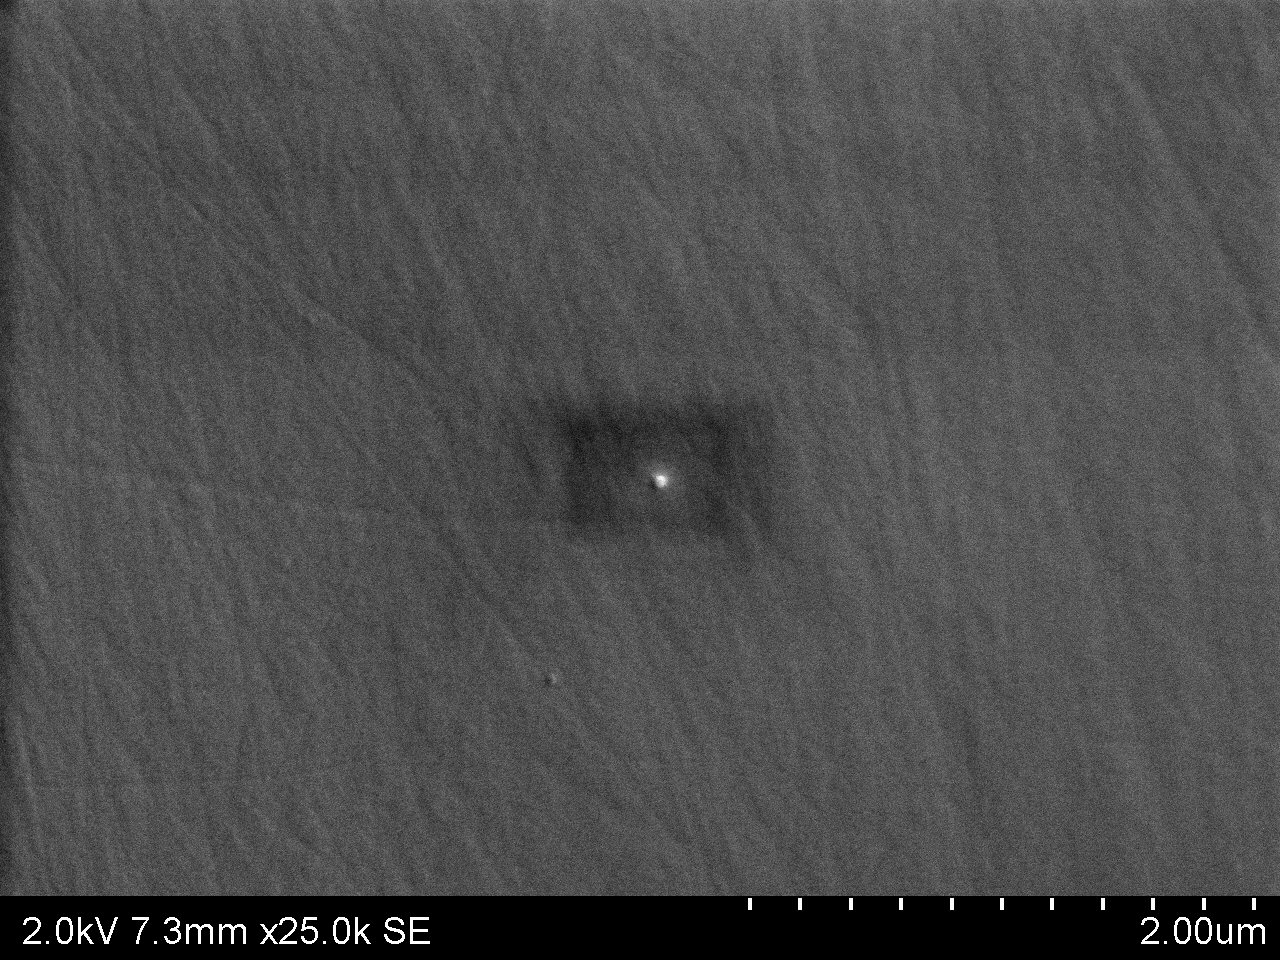
\includegraphics[width=0.6\linewidth]{substrateA_a1_m011.jpg}
    \caption[\Ac{sem} image of surface scratches on substrate A.]{High resolution \ac{sem} image of the surface of substrate A. The dark square was carbon deposited on the surface while focusing the beam at a higher magnification.}\label{fig:subAa_scratches}
    \label{fig:SEM_A_surface}
\end{figure}

The as-received substrate A was characterised for surface topography by \ac{afm}. Images of $\SI{5}{\micro\metre}\times\SI{5}{\micro\metre}$ areas were taken at three different locations on the substrate surface: near the centre, near the upper edge, and near the upper left corner, as seen in Fig.~\ref{fig:subAa_afm}. The \ac{rms} roughness of substrate A is \SI{\sim0.3}{\nano\metre} at both the centre and around the edges, while it is slightly higher at the corner with \iac{rms} roughness of \SI{\sim0.4}{\nano\metre}. This indicates the absence of large scratches. The typical surface scratches are between \SIrange{10}{20}{\nano\metre} wide and \SI{1}{\nano\metre} deep. While the largest polishing scratches are \SI{0.2}{\micro\metre} wide and \SI{5}{\nano\metre} deep.

\begin{figure}[htbp]
    \centering
    \begin{subfigure}[c]{0.032\linewidth}
        \label{fig:subAa_afm_scale}\captionsetup{list=no}
        
\includegraphics[width=\linewidth]{subAa_afm_scale.png}
    \end{subfigure}
    \hfill
    \mySubfigure{0.3\linewidth}{subAa_afm_centre.png}[fig:subAa_afm_centre]
    \hfill
    \mySubfigure{0.3\linewidth}{subAa_afm_upperedge.png}[fig:subAa_afm_edge]%0,26
    \hfill
    \mySubfigure{0.3\linewidth}{subAa_afm_upperleftcorner.png}[fig:subAa_afm_corner]%0,26
    \caption[\Ac{afm} of as-received substrate A.]{\Ac{afm} measurements of the as-received substrate A. Images of $\SI{5}{\micro\metre}\times\SI{5}{\micro\metre}$ areas are taken at three different locations on the substrate surface: \subref{fig:subAa_afm_centre} near the centre, \ac{rms} roughness \SI{0.31}{\nano\metre}; \subref{fig:subAa_afm_edge} near the upper edge, \ac{rms} roughness \SI{0.30}{\nano\metre}; and \subref{fig:subAa_afm_corner} near the upper left corner, \ac{rms} roughness \SI{0.41}{\nano\metre}.}\label{fig:subAa_afm}
\end{figure} % AFM, substrate A, as-received.

%%=========================================
%\section{Near-IR of As-Received Substrate A}

%%=========================================
\subsection{Impurity Analysis}

\Ac{xps} analysis was performed on the as-received substrate A to determine the composition of the outermost layers of the substrate (\SI{\sim 80}{\angstrom}). The centre of the $\SI{30}{\milli\metre}\times\SI{30}{\milli\metre}$ \ac{czt} wafer was analysed using \ac{xps}. With the large beam size of \SI{1}{\centi\metre}, it should be possible to see traces of impurity elements over a large area, but not locate them to specific particles or small areas. Unfortunately, something was broken on the old analyser, resulting in low signal intensity and no detection of impurities or small concentrations of elements. The ever-present oxide and carbon overlayers further decreased any small signals. Therefore, the XPS only gave information about the following elements: \ce{Te}, \ce{Cd}, \ce{O}, and \ce{C}, see Fig.~\ref{fig:xps_spectra}. The reason for not performing \ac{xps} analysis on substrate B was that it would not be possible to detect the presence of impurities or small concentrations of elements with the \ac{xps} equipment at hand.

\begin{figure}[htbp]
    \centering
    \mySubfigure{0.49\linewidth}{xps_Te3d.png}[fig:xps_Te3d]
    \hfill
    \mySubfigure{0.49\linewidth}{xps_Cd3d.png}[fig:xps_Cd3d]
    \par\bigskip
    \mySubfigure{0.49\linewidth}{xps_O1s.png}[fig:xps_O1s]
    \hfill
    \mySubfigure{0.49\linewidth}{xps_C1s.png}[fig:xps_C1s]
    \caption[\Ac{xps} spectra from substrate A.]{\Ac{xps} spectra from substrate A that displays the number of detected electrons (counts) as a function of their corresponding binding energy, $E_\mathrm{B}$ (\SI{}{\electronvolt}). The spectra were acquired using the \ce{Mg} anode. The peaks in the spectrum were: \subref{fig:xps_Te3d} \ce{Te} 3d with extra peaks due to tellurium oxide; \subref{fig:xps_Cd3d} \ce{Cd} 3d; \subref{fig:xps_O1s} \ce{O} 1s; and \subref{fig:xps_C1s} \ce{C} 1s.}
    \label{fig:xps_spectra}
\end{figure}
 
The atomic concentrations were calculated using Eq.~\eqref{eq:xps_concentration} with intensity peak areas and the following experimentally measured atomic sensitivity factors, determined earlier at \ac{ffi} \citep{hirsch1999x-ray}: \ce{Cd} 3d\textsubscript{5/2} (0.56), \ce{Te} 3d\textsubscript{5/2} (1.00), \ce{O} 1s (0.13), and \ce{C} 1s (0.05). Table~\ref{tab:xps_results} displays the results of the \ac{xps} analysis of substrate A. \ce{Cd_{0.96}Zn_{0.04}Te} should consist of \SI{48}{\atomic\percent} cadmium, \SI{2}{\atomic\percent} zinc and \SI{50}{\atomic\percent} tellurium, but zinc was not detected and the atomic concentration of \ce{Cd} was only \SI{75}{\percent} of that of \ce{Te} (it should be \SI{96}{\percent}). The higher than expected \ce{Te} concentration can be explained by the formation of a \ce{Te} oxide layer on the surface. By inserting the ratio between \ce{Te} in \ce{Cd_{1-y}Zn_yTe} signal and \ce{Te} in \ce{TeO} signal of \SI{1.3}{} into Eq.~\eqref{eq:signal_ratio}, the \ce{Te} oxide layer thickness was calculated to be \SI{0.96}{\nano\metre}. An atomic concentration of $23.5$ at.\% carbon was found, which can be explained by an overlayer of carbon. \todo{How thick?}

\begin{table}[htbp]
    \centering
    \caption[XPS analysis of the as-received substrate A.]{Results from the \ac{xps} analysis at the centre of the $30\times30$ \SI{}{\milli\metre} as-received (111)B \ce{CdZnTe} substrate A (atomic concentration \%).}\label{tab:xps_results}
    \begin{tabu} to 1.0\textwidth { X[1,c] X[1,c] X[1,c] X[1,c] X[1,c] }
    \hline
        %\textbf{$X$} (\SI{}{\milli\metre}) &  \textbf{$Y$} (\SI{}{\milli\metre}) & \textbf{\ce{Cd} (\SI{}{\atom\centi\metre^{-2}})} & \textbf{\ce{Te} (\SI{}{\atom\centi\metre^{-2}})} & \textbf{\ce{O} (\SI{}{\atom\centi\metre^{-2}})} & \textbf{\ce{C} (\SI{}{\atom\centi\metre^{-2}})} & \textbf{\ce{Te} oxide thickness (\SI{}{\nano\metre})}\\
        \textbf{\ce{Cd}}\newline(at.\%) & \textbf{\ce{Te}}\newline(at.\%) & \textbf{\ce{O} }\newline(at.\%) & \textbf{\ce{C}}\newline(at.\%) & \textbf{\ce{Te} oxide thickness}\newline(\SI{}{\nano\metre})\\
        \hline
         \SI{18.8}{} & \SI{25.1}{} & \SI{32.6}{} & \SI{23.5}{} & \SI{0.96}{} \\
         \hline
    \end{tabu}
\end{table}
%\mycomment{Add PeakFit-figures. Describe satellite peaks.}

%%=========================================
% EDS-analysis
Since the \ac{xps} equipment did not detect small concentrations of elements, \ac{eds} was used to get a quantitative analysis of the chemical composition of the substrate. The spectra were taken using an accelerating voltage of \SI{10.0}{\kilo\volt} to ensure the peaks of interest, a large probe current to maximise the throughput, and a live acquisition time of \SI{1200}{\second} to get good statistics (less noise). The results from the as-received substrate A can be seen in Table~\ref{tab:subAa_eds_analysis}. %an extraction voltage of \SI{2.00}{\kilo\volt} to get 

The electron interaction depth was calculated by the Quantax software to be \SI{0.4}{\micro\metre}. That means that characteristic X-rays from elements as far in as \SI{0.4}{\micro\metre} below the surface were detected. In comparison, the \ac{xps} detects the electrons that escape from the outermost \SI{\sim10}{\nano\metre}. Hence, \ac{eds} is not as surface sensitive and more than just the top surface layer is probed. This is part of the reason for the difference in the atomic concentrations between the \ac{xps} and \ac{eds} results for substrate A. The observed silica and alumina particles have a diameter of about \SI{50}{\nano\metre}. Hence, one monolayer of these would cover \SI{\sim12.5}{\percent} of the interaction volume, but more of the signal.

\begin{table}[htbp]
    \centering
    \caption[\Ac{eds} impurity analysis of the as-received substrate A.]{Results of the \ac{eds} impurity analysis at three different locations on the $30\times30$ \SI{}{\milli\metre^2} as-received (111)B \ac{czt} substrate A (atomic concentration \%). The X-ray signal is acquired from a $\SI{1270}{\micro\metre}\times\SI{890}{\micro\metre}$ area near the centre, upper edge, and upper left corner.}\label{tab:subAa_eds_analysis}
    \begin{tabu} to 1.0\textwidth { X[1.85,r] X[1.125,c] X[1.125,c] X[1.125,c] X[1.125,c] X[1.125,c] X[1.125,c] X[1.125,c] }
    \hline
         & \textbf{\ce{Te}} (at.\%) & \textbf{\ce{Cd}} (at.\%) & \textbf{\ce{Zn}} (at.\%) & \textbf{\ce{Al} } (at.\%) & \textbf{\ce{Si}} (at.\%) & \textbf{\ce{C}} (at.\%) & \textbf{\ce{O}} (at.\%) \\ % \textbf{$X$} (\SI{}{\milli\metre}) &  \textbf{$Y$} (\SI{}{\milli\metre})
        \hline
        Near centre  & \SI{45.94}{} & \SI{45.32}{} & \SI{1.98}{} & \SI{0.19}{} & \SI{0.45}{} & \SI{5.34}{} & \SI{0.78}{} \\ %\SI{15.0}{} & \SI{15.0}{}
        Near edge & \SI{46.14}{} & \SI{45.60}{} & \SI{1.90}{} & \SI{0.21}{} & \SI{0.51}{} & \SI{4.97}{} & \SI{0.68}{} \\ %\SI{15.0}{} & \SI{29.0}{}
        Near corner & \SI{46.05}{} & \SI{45.46}{} & \SI{1.89}{} & \SI{0.40}{} & \SI{0.51}{} & \SI{4.95}{} & \SI{0.73}{} \\ %\SI{1.0}{}  & \SI{29.0}{}
         \hline
    \end{tabu}
\end{table}

The \ac{eds} surface analysis identified the following elements: \ce{Cd}, \ce{Te}, \ce{Zn}, \ce{Al}, \ce{Si}, \ce{C}, and \ce{O}. The relative concentrations of \ce{Cd}, \ce{Zn}, and \ce{Te} had an error of less than one percentage point from the expected value of \SI{48}{\atomic\percent} cadmium, \SI{2}{\atomic\percent} zinc and \SI{50}{\atomic\percent} tellurium. There are detected silicon and alumina near the centre as well as near the edges and corners. This indicate that it is polishing grit in the centre as well. %\todo{Kan du si noe om density ut fra dette?}%Substrate A had a smaller atomic concentration of \ce{O} than substrate B, which indicates that the tellurium oxide layer on substrate A was thinner than that on substrate B. The \ce{Al} and \ce{Si} contamination found in the \ac{eds} analysis for both substrate A and substrate B was coming from residual \ce{Al2O3} and \ce{SiO2} polishing grit respectively.
%%========================================
% FTIR transmission spectra.
\subsection{IR Characterisation}

\Ac{ftir} transmission spectra were recorded from an $11\times11$ grid on the as-received substrate A. The grid points were placed \SI{2.0}{\milli\metre} from the edge and had \SI{2.6}{\milli\metre} between nearest neighbours. All but four measurements had an \ac{ir} transmittance between \SI{62}{\percent} and \SI{67}{\percent} in the wavenumber range between \SI{1000}{\centi\metre^{-1}} and \SI{5000}{\centi\metre^{-1}}, see Fig.~\ref{fig:subAa_ftir_spectra}. The spikes near $k=\SI{4500}{\centi\metre^{-1}}$ and $k=\SI{5000}{\centi\metre^{-1}}$ are an artefact of the \ac{ftir} instrument and should not be considered. A map of the transmission at $k=\SI{500}{\centi\metre^{-1}}$ can be seen in Fig.~\ref{fig:subAa_ftir_map_500cm-1}.

\begin{figure}[htbp]
    \centering
    \mySubfigure{0.60175438596\linewidth}{subAa_121_ftir_spectra.png}[fig:subAa_ftir_spectra]
    \hfill
    \mySubfigure{0.37824561403\linewidth}{subAa_121_ftir_transmission_at_k500cm-1.png}[fig:subAa_ftir_map_500cm-1]
    \caption[\Ac{ftir} measurements of the as-received substrate A.]{\Ac{ftir} measurements recorded from a $11\times11$ grid on the as-received $\SI{30}{\milli\metre}\times\SI{30}{\milli\metre}$ (111)B-oriented substrate A: \subref{fig:subAa_ftir_spectra} Transmission spectra; \subref{fig:subAa_ftir_map_500cm-1} transmission map at wavenumber $k=\SI{500}{\centi\metre^{-1}}$ showing the transmittance $T$ in percentage of incoming light that is transmitted through at each grid point. The spikes near $k=\SI{4500}{\centi\metre^{-1}}$ and $k=\SI{5000}{\centi\metre^{-1}}$ are an artefact of the \ac{ftir} instrument and should not be considered.}
\end{figure}

The two factors that are mainly responsible for the reduction in \ac{ir} transmittance of \ac{czt} are the free carrier absorption and the scattering effect of precipitates \citep{yadava1994precipitation}. \citet{yujie2004infrared} used the transmittance at the wavenumber of $\SI{1000}{\centi\metre^{-1}}$ $T_{1000}$, the transmittance at the wavenumber of $\SI{5000}{\centi\metre^{-1}}$ $T_{5000}$, and the ratio of $T_{1000}$ to $T_{5000}$ to determine which of these two mechanisms that are the most significant. Their analysis gives a qualitative determination of the density and size of \ce{Te} precipitates, the free carrier concentration, and the resistivity for \ac{czt} substrates. %\todo{Espen: Dislokasjoner og ruhet vil også senke transmisjon.}

Almost all the spectra from substrate A had a value of $T_{5000}$ between \SI{63}{\percent} and \SI{67}{\percent}, $T_{1000}$ between \SI{62}{\percent} and \SI{64}{\percent}, and $T_{1000}/T_{5000}$ approaches one from below. According to \citet{yujie2004infrared}, the \ac{czt} substrates with these characteristics are free of precipitates, have low free carrier concentration, and have resistivity that exceeds \SI{e6}{\ohm\centi\metre}.%\todo{Why?}
%%========================================
